This chapter will present the results and discussion divided into six consecutive themes: general performance, gaming effects, task load index, subjective delay, learning effects and key presses.

\section{Performance}

\figref{performanceNorm} shows the normalized number of hits in 90 seconds (score), for each display type and all N=57 participants. \textit{Delay} refers to the \textit{added} delay, which means that "No delay" translates to the inherent system delay of $250 ms$. The numerical values are reported in Table \ref{score}. The statistical significance and effect size between conditions can be seen in Table \ref{score2}.

\begin{figure}[h!]
    \centering
    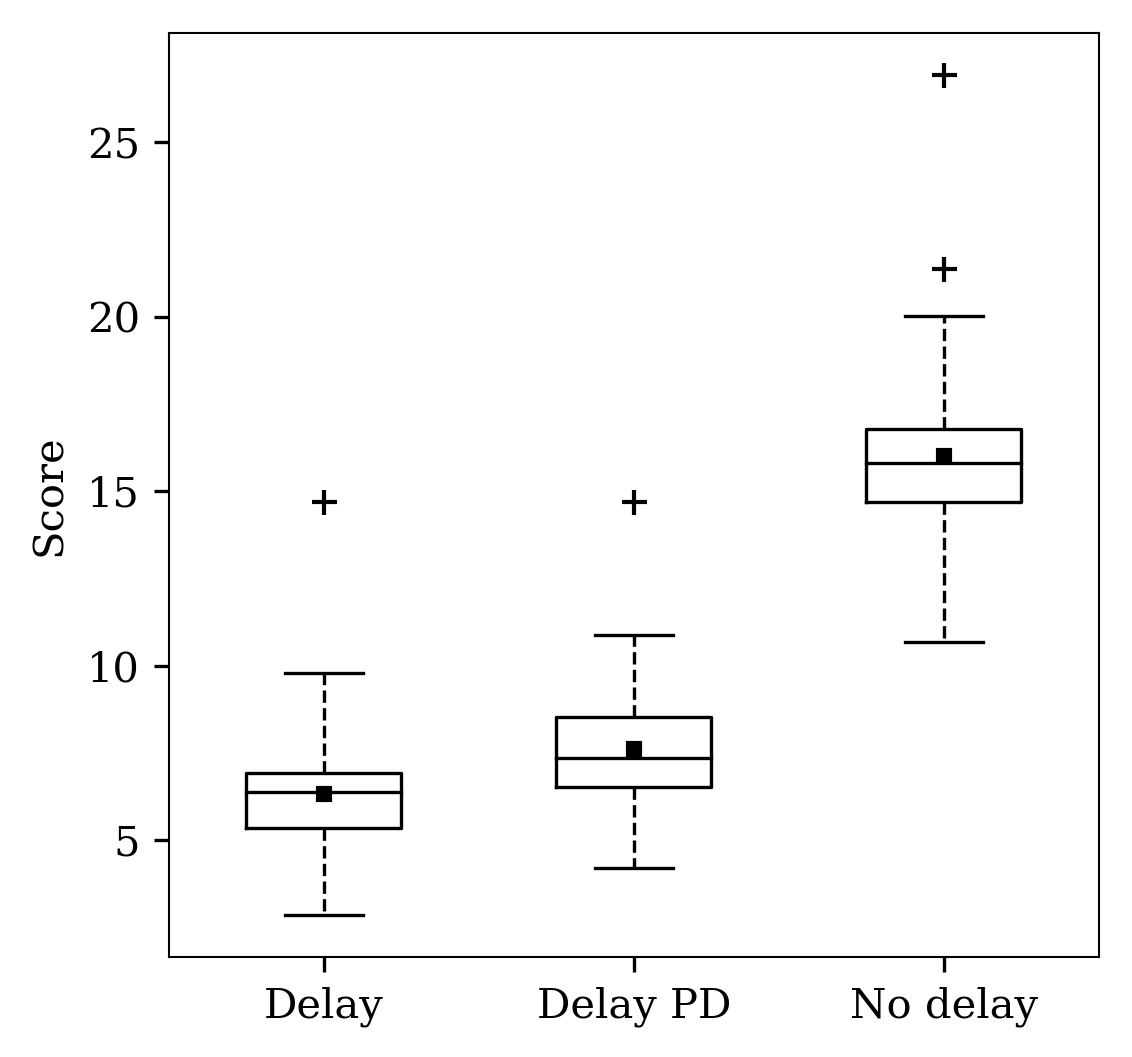
\includegraphics[scale=0.85]{performance_norm}
    \caption{Normalized score all participants, N=57.}
    \label{performanceNorm}
	\vspace{-0.2cm}
\end{figure}

% Please add the following required packages to your document preamble:
% \usepackage{booktabs}
\begin{table}[]
\small
\centering
\caption{Normalized mean scores and standard deviation (SD).}
\label{score}
\begin{tabularx}{\textwidth}{@{}XXXXX@{}}
\toprule
Differentiation & Group       & Display  & Score & SD \\ \midrule
None            & All N=57    & Delay    & 6.24  & 1.39               \\
                &             & Delay PD & 7.52  & 1.43               \\
                &             & No delay & 15.87 & 1.99               \\ \addlinespace
Gender          & Male n=38   & Delay    & 6.65  & 1.25               \\
                &             & Delay PD & 7.95  & 1.43               \\
                &             & No delay & 17.30 & 1.71               \\ \addlinespace
                & Female n=19 & Delay    & 5.39  & 1.49               \\
                &             & Delay PD & 6.61  & 1.35               \\
                &             & No delay & 13.10 & 2.17               \\ \addlinespace
Gaming          & Daily n=2   & Delay    & 7.92  & 0.37               \\
                &             & Delay PD & 10.21 & 1.40               \\
                &             & No delay & 18.36 & 1.77               \\ \addlinespace
                & Weekly n=15 & Delay    & 6.27  & 1.22               \\
                &             & Delay PD & 8.17  & 1.51               \\
                &             & No delay & 17.62 & 2.04               \\ \addlinespace
                & Monthly n=8 & Delay    & 7.05  & 1.32               \\
                &             & Delay PD & 7.77  & 0.64               \\
                &             & No delay & 17.68 & 0.95               \\ \addlinespace
                & Yearly n=17 & Delay    & 6.65  & 1.26               \\
                &             & Delay PD & 7.66  & 1.73               \\
                &             & No delay & 15.98 & 2.25               \\ \addlinespace
                & Never n=15  & Delay    & 5.06  & 1.46               \\
                &             & Delay PD & 6.21  & 1.16               \\
                &             & No delay & 12.73 & 1.79               \\ \bottomrule
\end{tabularx}
\end{table}

% Please add the following required packages to your document preamble:
% \usepackage{booktabs}
\begin{table}[]
\centering
\caption{Paired samples t-test and Cohen's d effect size}
\label{score2}
\begin{tabularx}{\textwidth}{@{}llYYYY@{}}
\toprule
\multicolumn{2}{c}{Pair} & \multicolumn{3}{c}{t-test for Equality of Means} &       \\ \cmidrule(lr){3-5}
\multicolumn{2}{l}{}     & t                  & df             & p                   & d     \\ \midrule
Delay       & Delay PD   & 4.82               & 56             & $<$.001             & 0.735 \\
Delay       & No delay   & 23.04              & 56             & $<$.001             & 4.413 \\
Delay PD    & No delay   & 19.52              & 56             & $<$.001             & 3.861 \\ \bottomrule
\end{tabularx}
\end{table}

\figref{performanceNorm} together with the statistical data in Table \ref{score2} shows that there is a statistical difference in performance when controlling the ROV without and with predictive help. Subjects performed on average 20.6\% better with an effect size of $d=0.904$. This can be categorized as a medium to large effect, especially when considering how easy and cheap this predictive method is to implement.

Past research, Table \ref{reviewPred}, describes a wide range performance gains from predictive technology. Everything from 8\% to 65\%. It's hard to do a direct comparison to any specific experiment, but a performance increase of 20.6\% in this experiment is probably in the lower range of what has been found before. What is true though, is that the predictive method described in this thesis is the cheapest and easiest to implement, at least when comparing to those in Table \ref{reviewPred}.

None of the subjects were told that there would be a predictive display or how it worked. Some of the participants immediately identified what the predictive display was trying to tell them. Others however, didn't understand that there had been a predictive display until the experiment was over. The ones who tried to use the predictive display the way it was intended typically performed better than those who didn't. It may be possible that we could have seen an improved performance, if the subjects were informed how the predictive display works. This can however not be verified unless additional experiments are performed.

\section{Gaming}

Those who play games weekly or more were defined as \emph{gamers} (G). They performed on average 30.13\% better, while non-gamers (NG) only saw a 16.91\% performance increase using the PD. This difference is illustrated in \figref{gamer_performance} and Table \ref{score2}.

\begin{figure}[h!]
    \centering
    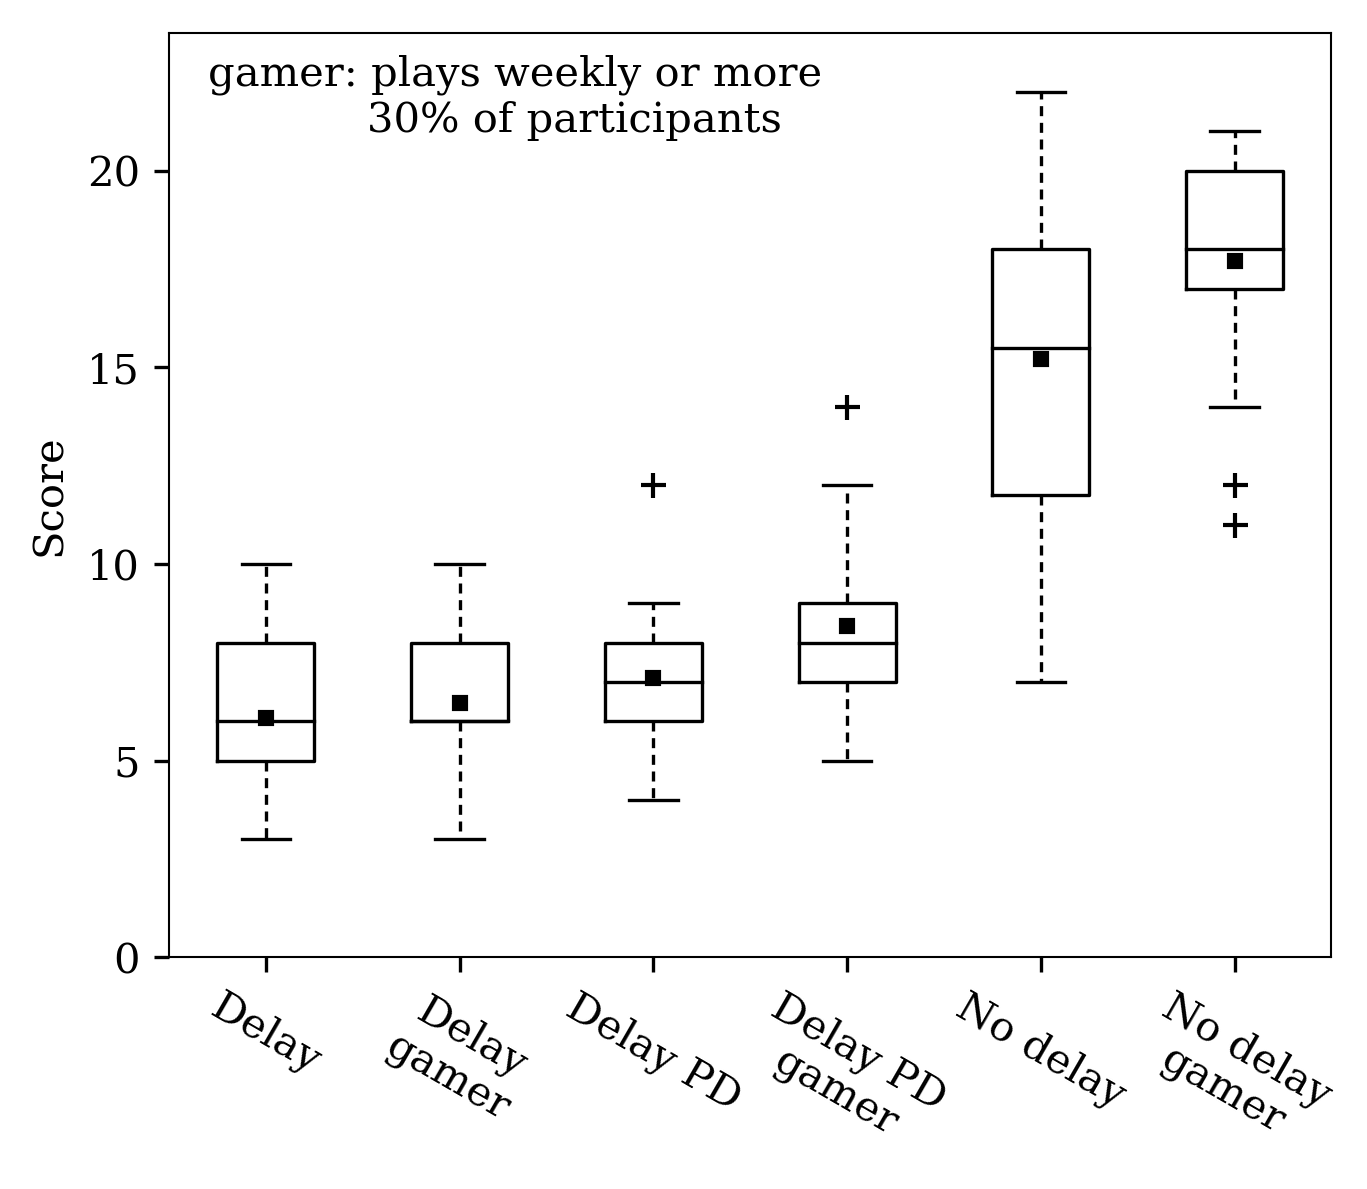
\includegraphics[scale=0.85]{gamer_performance}
    \caption{Performance of gamers n=17, versus non-gamers n=40.}
    \label{gamer_performance}
\end{figure}

It is interesting to see that G's were able to increase their score almost twice as much as NG's when going from a delayed condition to a delayed condition with PD. Exactly why G's were able to increase their performance more using the PD is unclear. It could be that the arrow in the PD which acts like an aiming device, is a more familiar concept for gamers. It could also indicate that G's are generally more adaptable to new an unfamiliar situations in a computer competition setting.

When comparing G's versus NG's directly, it is also interesting to see that G's only performed better than NG's in the second and third condition. Delay PD: t(26.57)=2.23, p=0.034, d=0.692 and no delay: t(40.79)=2.56, p=0.014, d=0.660. In the the first condition, there was no significant difference.
\todo[inline]{
why is this
}
This tells us that G's were only able to utilize their potential if there was 


\section{Task load index}

\figref{tlx} shows the reported NASA TLX scores. The height of the bar describes the mean value while the whiskers shows the SD. Numerical values are reported in Table \ref{tlx_values}.

Subjects reported minimal differences between condition one and two. The only significant differences were found in performance and frustration. Subjects felt that they on average performed 14\% better using the predictor display, t(56)=3.24, p=0.002, d=0.360. The actual performance increase was 21\%. They also reported that they felt 11\% less frustrated using the PD, t(56)=2.15, p=0.036, d=0.271. Participants also stated that the no delay condition was better in all metrics, with an exception of \emph{temporal demand} where the difference was not significant.

\begin{figure}[h!]
    \centering
    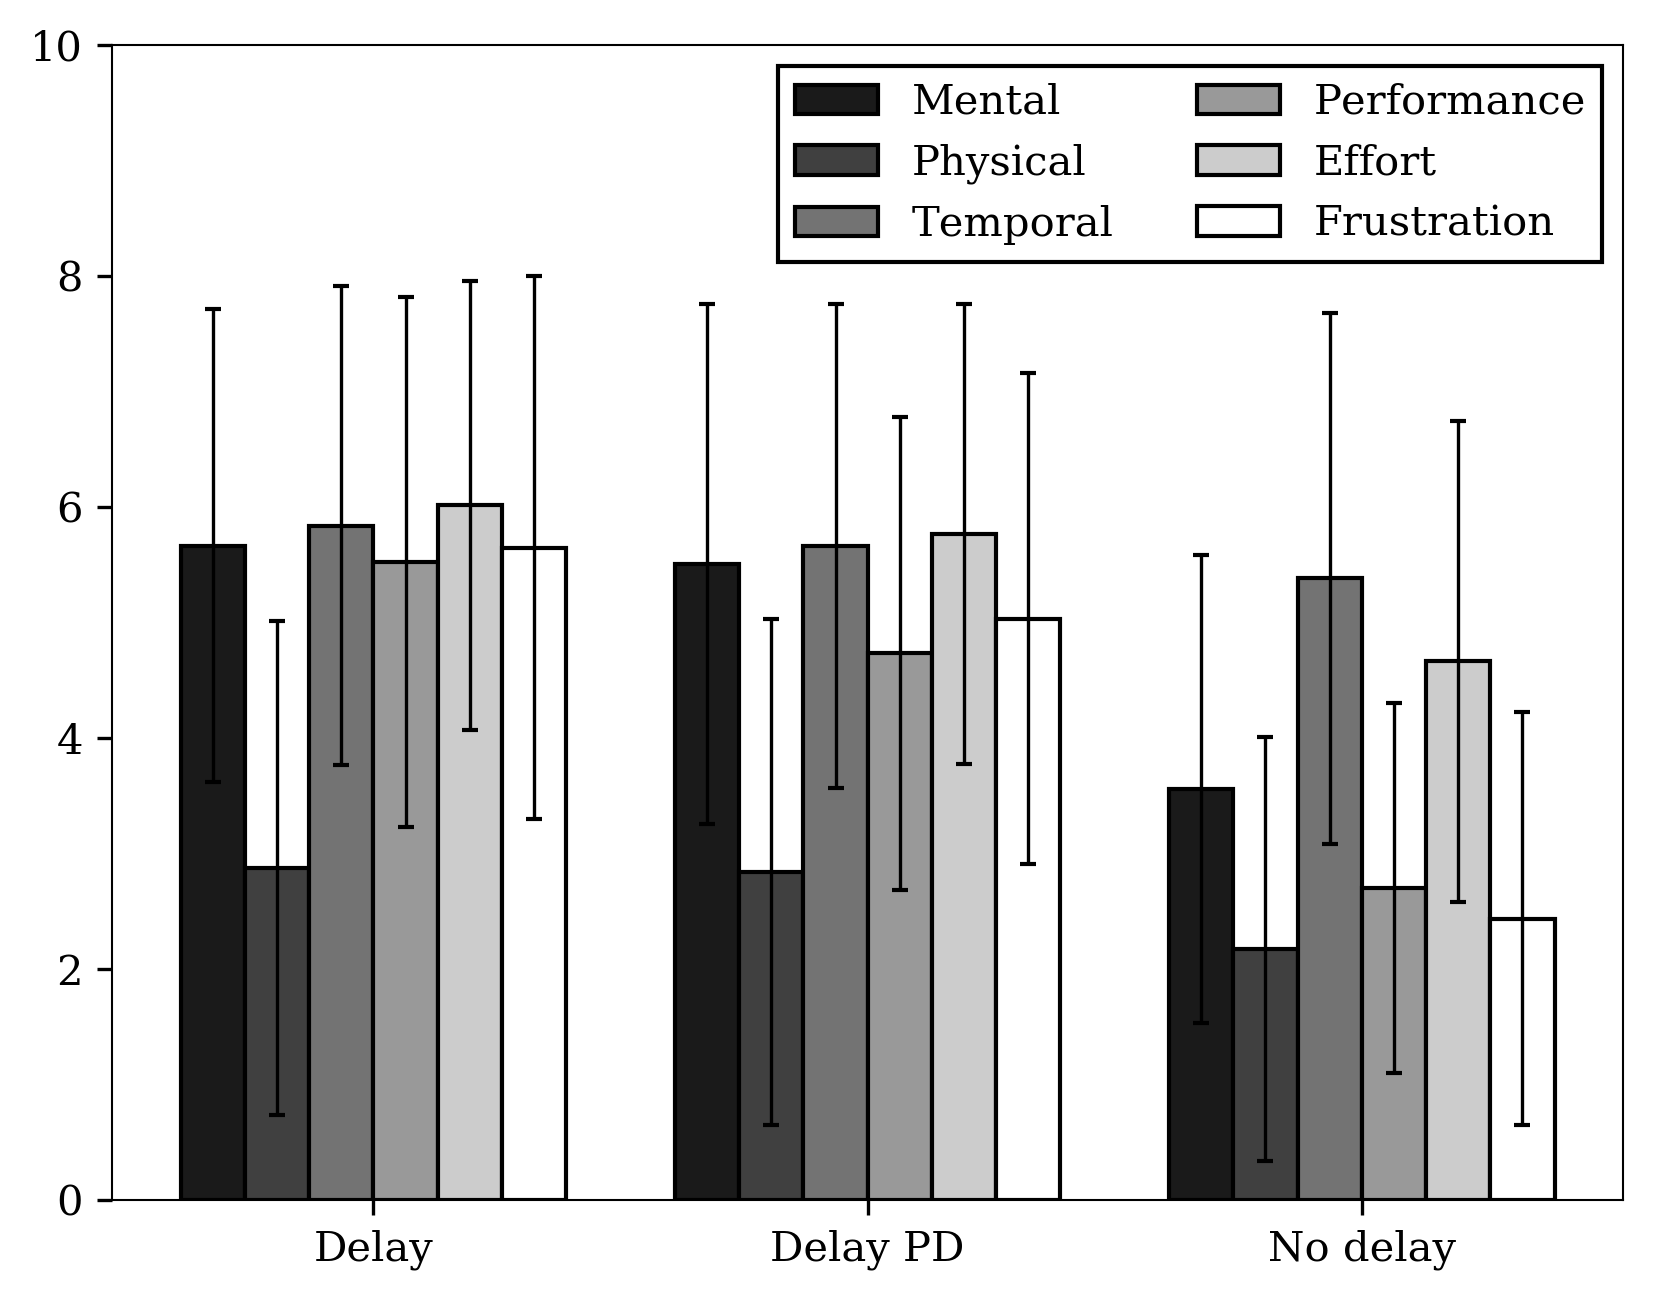
\includegraphics[scale=0.85]{nasa_tlx_bar}
    \caption{NASA TLX (task load index) results for each display type, N=57. Lower is better.}
    \label{tlx}
\end{figure}

% Please add the following required packages to your document preamble:
% \usepackage{booktabs}
\begin{table}[]
\small
\centering
\caption{Rated NASA TLX values and standard deviation (SD), N=57. Lower is better.}
\label{tlx_values}
\begin{tabularx}{\textwidth}{@{}XXXX@{}}
\toprule
Metric      & Display  & Rated value & SD \\ \midrule
Mental      & Delay    & 5.67        & 2.05               \\
            & Delay PD & 5.51        & 2.25               \\
            & No delay & 3.56        & 2.03               \\\addlinespace
Physical    & Delay    & 2.88        & 2.14               \\
            & Delay PD & 2.84        & 2.19               \\
            & No delay & 2.18        & 1.84               \\\addlinespace
Temporal    & Delay    & 5.84        & 2.08               \\
            & Delay PD & 5.67        & 2.10               \\
            & No delay & 5.39        & 2.30               \\\addlinespace
Performance & Delay    & 5.53        & 2.29               \\
            & Delay PD & 4.74        & 2.05               \\
            & No delay & 2.70        & 1.60               \\\addlinespace
Effort      & Delay    & 6.02        & 1.94               \\
            & Delay PD & 5.77        & 1.99               \\
            & No delay & 4.67        & 2.08               \\\addlinespace
Frustration & Delay    & 5.65        & 2.35               \\
            & Delay PD & 5.04        & 2.13               \\
            & No delay & 2.44        & 1.79               \\ \bottomrule
\end{tabularx}
\end{table}

The subjects reported no significant difference in mental, physical and temporal demand between condition one and two. These three metrics is a good description of the total subjective workload. Some subjects, especially those who didn't understand what the PD were trying to tell them, even reported the PD as distracting. Because of how the PD works, the video feed is constantly moving around and scaling up and down. This can understandably be distracting. Some participants immediately understood how the PD worked, and they typically reported the PD as helpful. They also seemed to be more relaxed, but there are no recorded data that can prove this relationship.

During the task, a red timer indicating the remaining time was constantly visible for the participant to see in the upper right corner. In addition, the robot had rapid acceleration and was able move fast if the operator managed to do so. Overall, this made for a hectic and exiting experience for the subjects. This may explain why there is no significant change in the temporal demand, even compared to the no delay situation. The fact that the participants reported a better value (smaller) in the other five metrics for the no delay condition, is as expected. This finding supports earlier research that describes how video latency negatively affect the user experience in teleoperation.


\section{Subjective delay}

\figref{subjective_delay_norm} shows the normalized reported total delay in seconds for the three conditions. The participants reported a 11\% decrease in subjective latency using the predictive display versus the normal display with the same latency. This results is however not significant, t(56)=1.40, p=0.167, d=0.356.

\begin{figure}[h!]
    \centering
    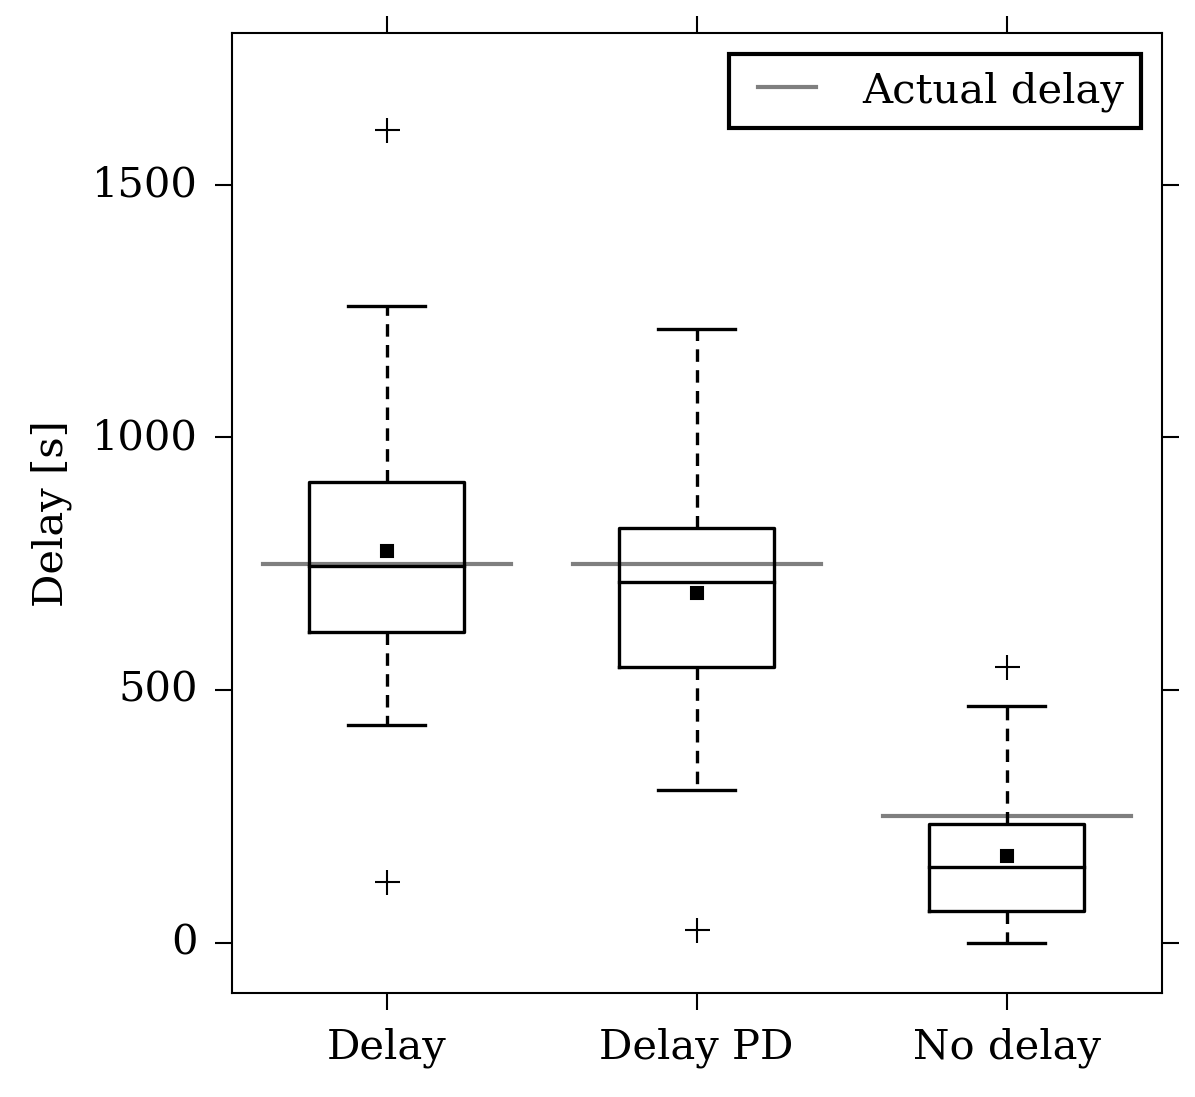
\includegraphics[scale=0.85]{subjective_delay_norm}
    \caption{Normalized reported subjective latency in seconds.}
    \label{subjective_delay_norm}
\end{figure}

Since the participants reported less frustration using the PD, it it interesting to look at how frustration an subjective delay time might be related. \figref{delay_vs_frustration} shows a scatter plot of reported frustration and delay time for all conditions collectively. All values has been normalized. The linear relationship is minimal at best and no conclusions can be drawn from the data.

\begin{figure}[h!]
    \centering
    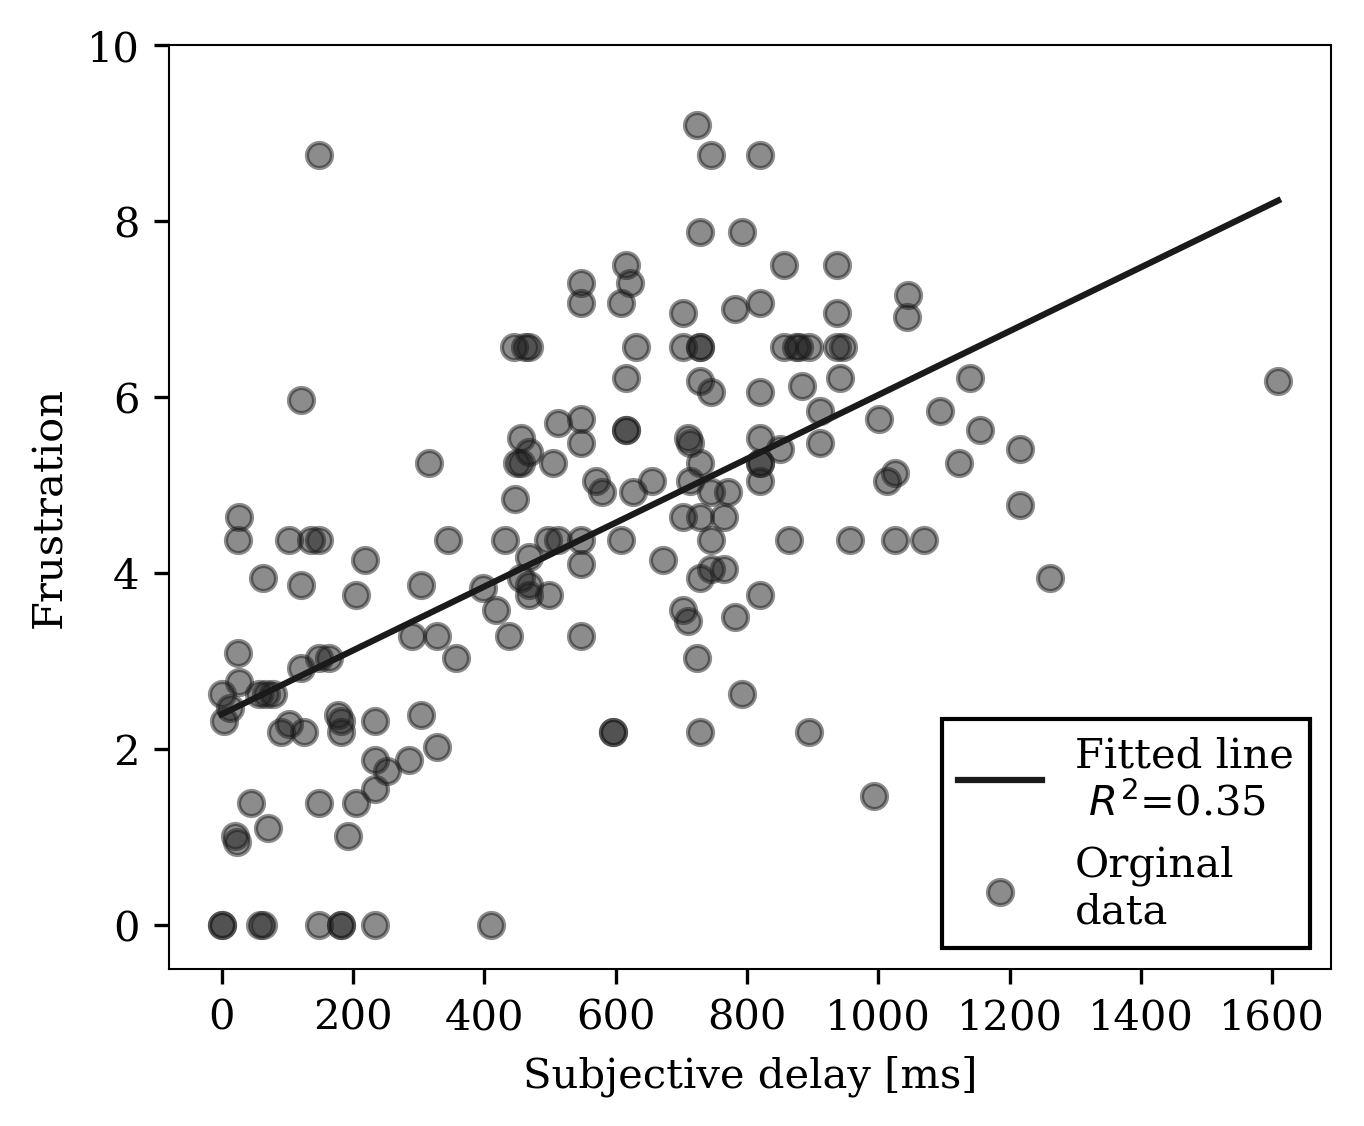
\includegraphics[scale=0.65]{delay_vs_frustration}
    \caption{Normalized subjective delay versus frustration}
    \label{delay_vs_frustration}
\end{figure}

\section{Learning effect}

It is also interesting the evaluate if participants had any learning effects during the experiment. \figref{learning_effect} shows the score for each display type and further divided into groups depending if the subject had that display as the first, second or third display. As an example, the first of the nine box plots describes the score achieved in the delay condition for those who had that display as their first display. One visible trend is that the participants who had a particular display as their second display, performed better than those who had that display as their first. This performance increase was significant for all displays. Delay: t(18)=2.19, p=0.042, d=0.671, delay PD: t(17)=2.19, p=0.043, d=0.660, no delay: t(17)=3.26, p=0.005, d=0.902. The performance change from \#2 to \#3 in all displays were however not found significant.

\begin{figure}[h!]
    \centering
    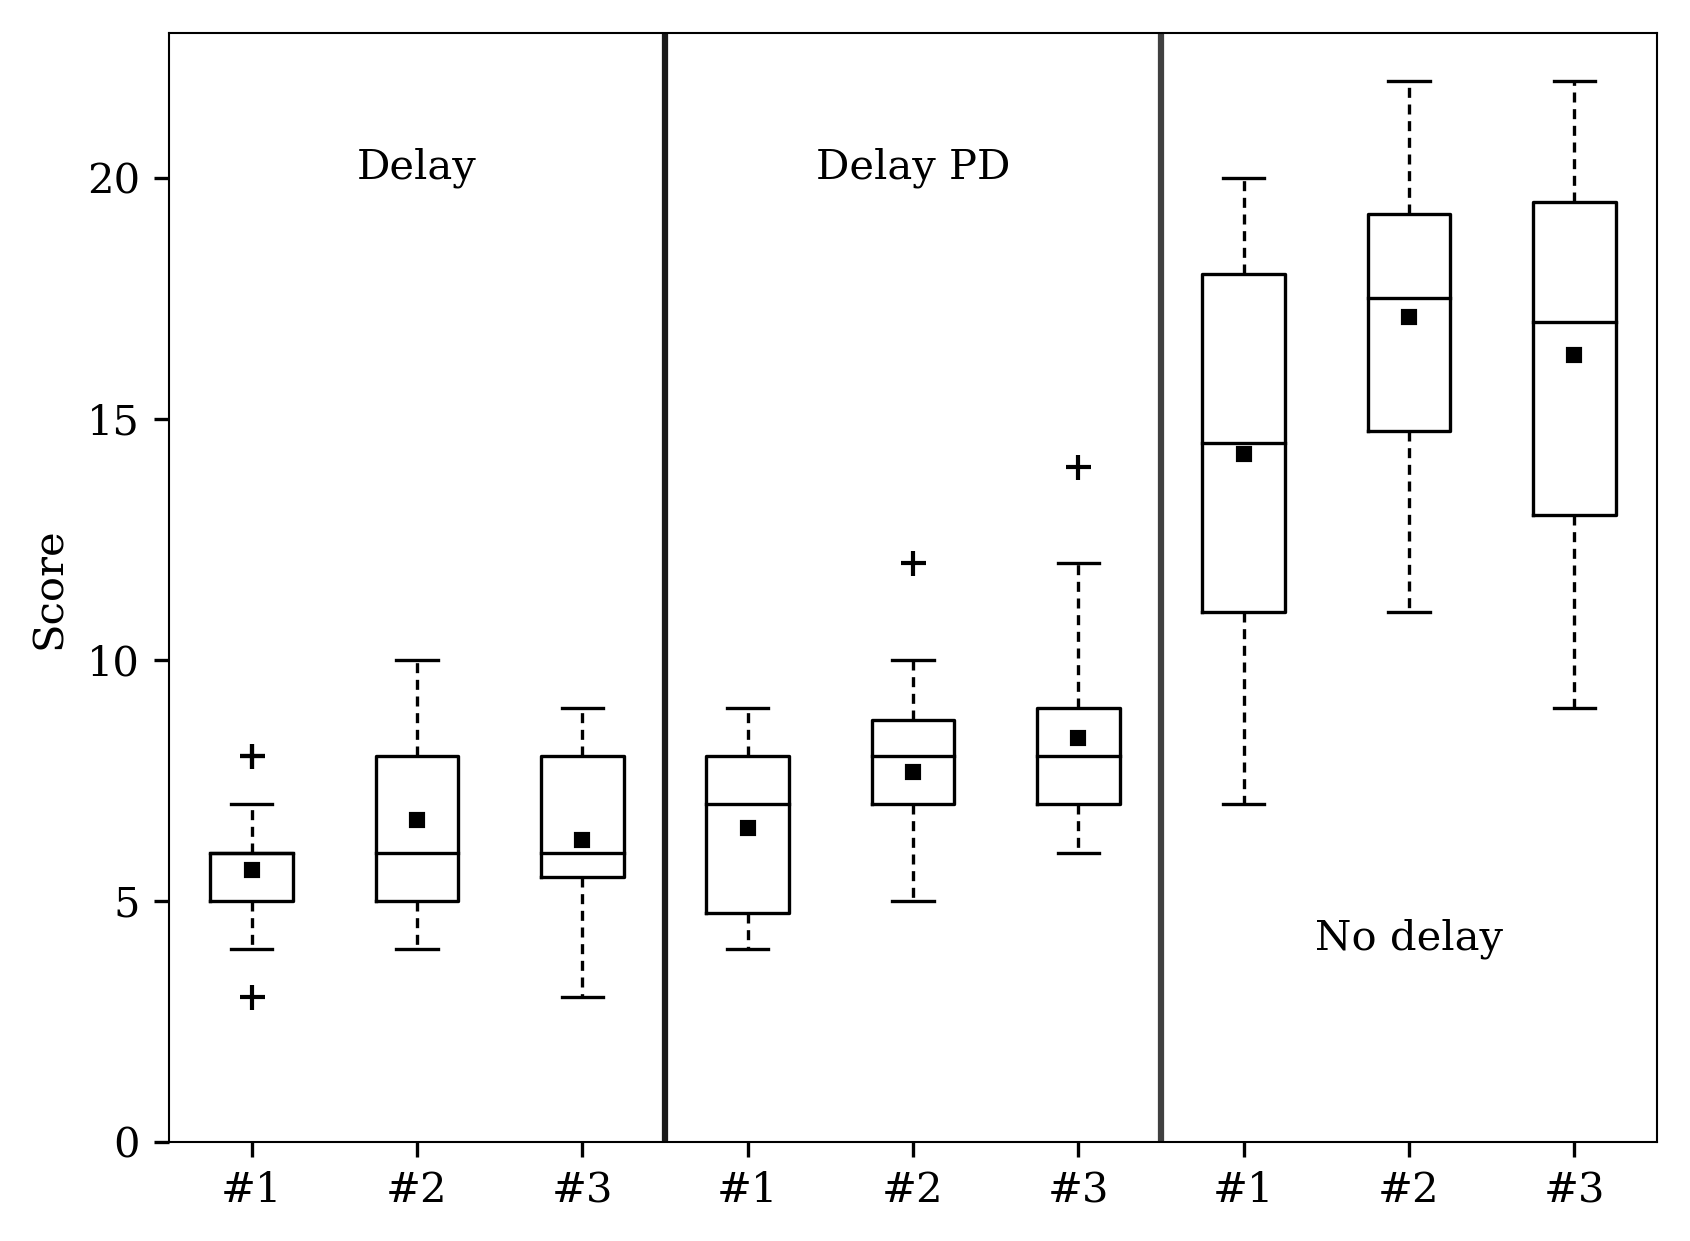
\includegraphics[width=0.7\textwidth]{learning_effect}
    \caption{Score categorized after display order.}
    \label{learning_effect}
\end{figure}

\section{Key presses}

\figref{keypresses} shows the number of key presses performed during the 90 seconds of task time for each display type. With a low latency, participants are in a greater degree trying to continuously maneuver the ROV.

\begin{figure}[h!]
    \centering
    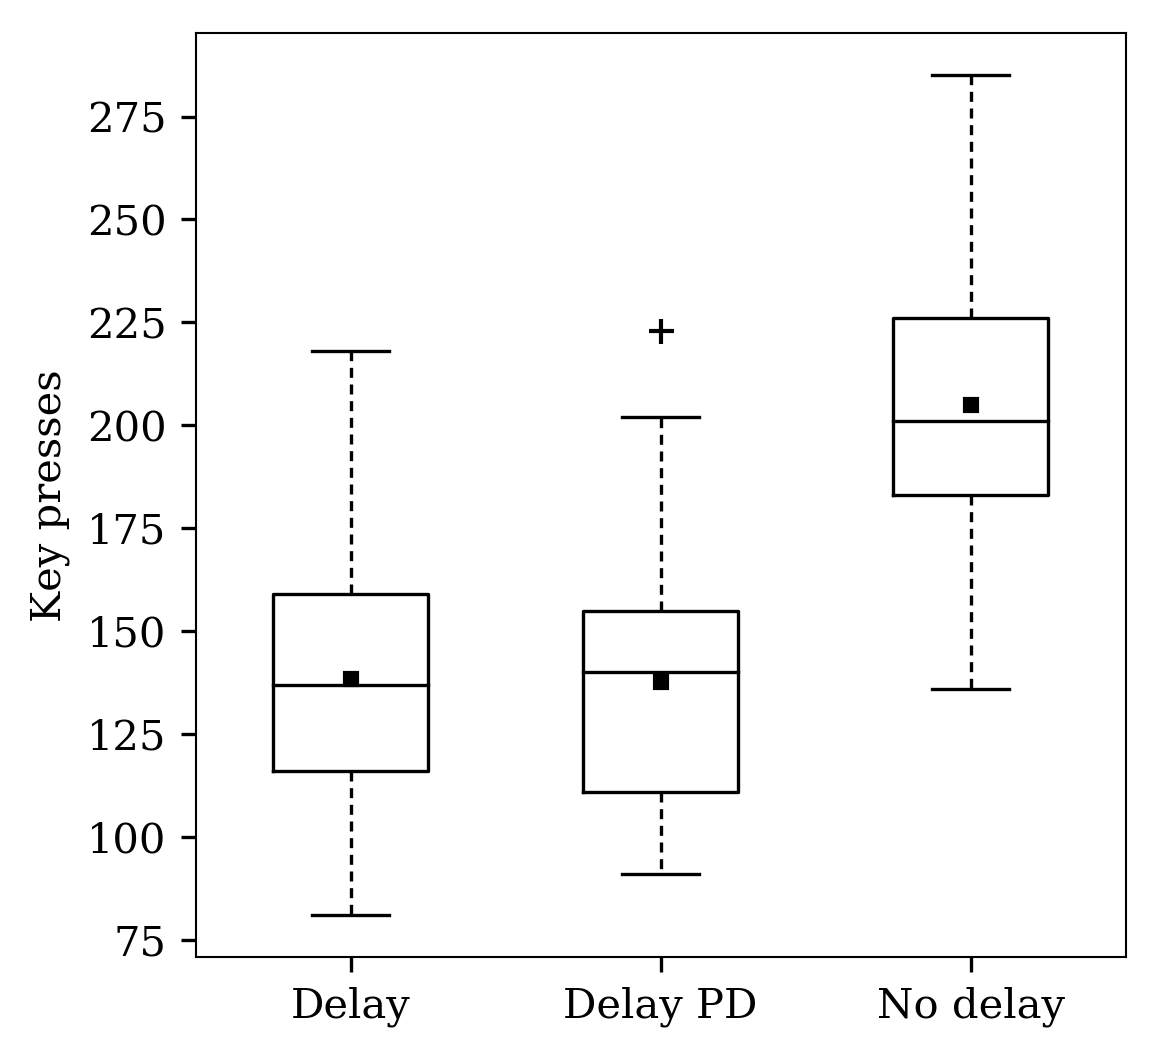
\includegraphics[scale=0.85]{keypresses}
    \caption{The number of key presses performed during 90 seconds.}
    \label{keypresses}
\end{figure}
